\documentclass[uplatex, dvipdfmx]{jsarticle}
    
\title{生命科学レポート}
\author{司馬博文 J4-190549}
\date{\today}
\pagestyle{headings} \setcounter{secnumdepth}{4}
\usepackage{amsmath, amsfonts, amsthm, amssymb, ascmac, color, comment, wrap fig}

\usepackage{mathtools}
\mathtoolsset{showonlyrefs=true} %labelを附した数式にのみ附番される.

\usepackage{tikz, tikz-cd}
\usepackage[all]{xy}
\def\objectstyle{\displaystyle} %デフォルトではxymatrix中の数式が文中数式モードになるので,それを直した.

%化学式をTikZで簡単に書くためのパッケージ.
\usepackage[version=4]{mhchem} %texdoc mhchem
%化学構造式をTikZで描くためのパッケージ.
\usepackage{chemfig}
%IS単位を書くためのパッケージ
\usepackage{siunitx}
%取り消し線を引くためのパッケージ
\usepackage{ulem}

%\rotateboxコマンドを,文字列の中心で回転させるオプション.
%他rotatebox, scalebox, reflectbox, resizeboxなどのコマンド.
\usepackage{graphicx}

%加藤晃史さんがフル活用していたtcolorboxを,途中改ページ可能で.
\usepackage[breakable]{tcolorbox}

%enumerate環境を凝らせる.
\usepackage{enumerate}

%日本語にルビをふる
\usepackage{pxrubrica}

%足助さんからもらったオプション
%\usepackage[shortlabels,inline]{enumitem}
%\usepackage[top=15truemm,bottom=15truemm,left=10truemm,right=10truemm]{geometry}

%以下,ソースコードを表示する環境の設定.
\usepackage{listings,jvlisting} %日本語のコメントアウトをする場合jlistingが必要
%ここからソースコードの表示に関する設定
\lstset{
  basicstyle={\ttfamily},
  identifierstyle={\small},
  commentstyle={\smallitshape},
  keywordstyle={\small\bfseries},
  ndkeywordstyle={\small},
  stringstyle={\small\ttfamily},
  frame={tb},
  breaklines=true,
  columns=[l]{fullflexible},
  numbers=left,
  xrightmargin=0zw,
  xleftmargin=3zw,
  numberstyle={\scriptsize},
  stepnumber=1,
  numbersep=1zw,
  lineskip=-0.5ex
}
%lstlisting環境で,[caption=hoge,label=fuga]などのoptionを付けられる.
\makeatletter
    \AtBeginDocument{
    \renewcommand*{\thelstlisting}{\arabic{chapter}.\arabic{section}.\arabic{lstlisting}}
    \@addtoreset{lstlisting}{section}
    }
\makeatother
%caption番号を「[chapter番号].[section番号].[subsection番号]-[そのsubsection内においてn番目]」に変更
\renewcommand{\lstlistingname}{program}
%caption名を"program"に変更

%%%
%%%フォント
%%%

%本文・数式の両方のフォントをTimesに変更するお手軽なパッケージだが,LaTeX標準数式記号の\jmath, \amalg, coprodはサポートされない.
% \usepackage{mathptmx}
%Palatinoの方が完成度が高いと美文書作成に書いてあった.
\usepackage[sc]{mathpazo} %オプションは,familyの指定.pplxにしている.
%2000年のYoung Ryuによる新しいTimes系.なおPalatinoもある.
% \usepackage{newtxtext, newtxmath}
%拡張数学記号.\textsectionでブルバキに!
\usepackage{textcomp, mathcomp}
\usepackage[T1]{fontenc} %8bitエンコーディングにする.comp系拡張数学文字の動作が安定する.
%AMS Euler.Computer Modernと相性が悪いとは…….
\usepackage{ccfonts, eulervm} %KnuthのConcrete Mathematicsの組み合わせ.
% \renewcommand{\rmdefault}{pplx} %makes LaTeX use Palatino in place of CM Roman.Do not use the Euler math fonts in conjunction with the default Computer Modern text fonts – this is ugly!

%%% newcommands
    %参考文献で⑦というのを出したかった.\circled{n}と打てば良い.LaTeX StackExchangeより.
\newcommand*\circled[1]{\tikz[baseline=(char.base)]{\node[shape=circle,draw,inner sep=0.8pt] (char) {#1};}}

%%%
%%% ショートカット 足助さんからのコピペ
%%%

\DeclareMathOperator{\grad}{\mathrm{grad}}
\DeclareMathOperator{\rot}{\mathrm{rot}}
\DeclareMathOperator{\divergence}{\mathrm{div}}
\newcommand\R{\mathbb{R}}
\newcommand\N{\mathbb{N}}
\newcommand\C{\mathbb{C}}
\newcommand\Z{\mathbb{Z}}
\newcommand\Q{\mathbb{Q}}
\newcommand\GL{\mathrm{GL}}
\newcommand\SL{\mathrm{SL}}
\newcommand\False{\mathrm{False}}
\newcommand\True{\mathrm{True}}
\newcommand\tr{\mathrm{tr}}
\newcommand\M{\mathcal{M}}
\newcommand\F{\mathbb{F}}
% \newcommand\H{\mathbb{H}} すでにある.
\newcommand\id{\mathrm{id}}
\newcommand\A{\mathcal{A}}
%\renewcommand\coprod{\rotatebox[origin=c]{180}{$\prod$}}
\newcommand\pr{\mathrm{pr}}
\newcommand\U{\mathfrak{U}}
\newcommand\Map{\mathrm{Map}}
\newcommand\dom{\mathrm{dom}}
\newcommand\cod{\mathrm{cod}}
\newcommand\supp{\mathrm{supp}}
%%% 複素解析学
\renewcommand\Re{\mathrm{Re}\;}
\renewcommand\Im{\mathrm{Im}\;}
\newcommand\Gal{\mathrm{Gal}}
\newcommand\PGL{\mathrm{PGL}}
\newcommand\PSL{\mathrm{PSL}}
%%% 解析力学
\newcommand\x{\mathbf{x}}
\newcommand\q{\mathbf{q}}
%%% 集合と位相
\newcommand\ORD{\mathrm{ORD}}

%%% 圏
\newcommand\Hom{\mathrm{Hom}}
\newcommand\Mor{\mathrm{Mor}}
\newcommand\Aut{\mathrm{Aut}}
\newcommand\End{\mathrm{End}}
\newcommand\op{\mathrm{op}}
\newcommand\ev{\mathrm{ev}}
\newcommand\Ob{\mathrm{Ob}}
\newcommand\Ar{\mathrm{Ar}}
\newcommand\Arr{\mathrm{Arr}}
\newcommand\Set{\mathrm{Set}}
\newcommand\Grp{\mathrm{Grp}}
\newcommand\Cat{\mathrm{Cat}}
\newcommand\Mon{\mathrm{Mon}}
\newcommand\CMon{\mathrm{CMon}}
\newcommand\Pos{\mathrm{Pos}}
\newcommand\Vect{\mathrm{Vect}}
\newcommand\FinVect{\mathrm{FinVect}}
\newcommand\Fun{\mathrm{Fun}}
\newcommand\Ord{\mathrm{Ord}}

%%%
%%% 定理環境 以下足助さんからのコピペ
%%%

\newtheoremstyle{StatementsWithStar}% ?name?
{3pt}% ?Space above? 1
{3pt}% ?Space below? 1
{}% ?Body font?
{}% ?Indent amount? 2
{\bfseries}% ?Theorem head font?
{\textbf{.}}% ?Punctuation after theorem head?
{.5em}% ?Space after theorem head? 3
{\textbf{\textup{#1~\thetheorem{}}}{}\,$^{\ast}$\thmnote{(#3)}}% ?Theorem head spec (can be left empty, meaning ‘normal’)?
%
\newtheoremstyle{StatementsWithStar2}% ?name?
{3pt}% ?Space above? 1
{3pt}% ?Space below? 1
{}% ?Body font?
{}% ?Indent amount? 2
{\bfseries}% ?Theorem head font?
{\textbf{.}}% ?Punctuation after theorem head?
{.5em}% ?Space after theorem head? 3
{\textbf{\textup{#1~\thetheorem{}}}{}\,$^{\ast\ast}$\thmnote{(#3)}}% ?Theorem head spec (can be left empty, meaning ‘normal’)?
%
\newtheoremstyle{StatementsWithStar3}% ?name?
{3pt}% ?Space above? 1
{3pt}% ?Space below? 1
{}% ?Body font?
{}% ?Indent amount? 2
{\bfseries}% ?Theorem head font?
{\textbf{.}}% ?Punctuation after theorem head?
{.5em}% ?Space after theorem head? 3
{\textbf{\textup{#1~\thetheorem{}}}{}\,$^{\ast\ast\ast}$\thmnote{(#3)}}% ?Theorem head spec (can be left empty, meaning ‘normal’)?
%
\newtheoremstyle{StatementsWithCCirc}% ?name?
{6pt}% ?Space above? 1
{6pt}% ?Space below? 1
{}% ?Body font?
{}% ?Indent amount? 2
{\bfseries}% ?Theorem head font?
{\textbf{.}}% ?Punctuation after theorem head?
{.5em}% ?Space after theorem head? 3
{\textbf{\textup{#1~\thetheorem{}}}{}\,$^{\circledcirc}$\thmnote{(#3)}}% ?Theorem head spec (can be left empty, meaning ‘normal’)?
%
\theoremstyle{definition}
 \newtheorem{theorem}{定理}[section]
 \newtheorem{axiom}[theorem]{公理}
 \newtheorem{corollary}[theorem]{系}
 \newtheorem{proposition}[theorem]{命題}
 \newtheorem*{proposition*}{命題}
 \newtheorem{lemma}[theorem]{補題}
 \newtheorem*{lemma*}{補題}
 \newtheorem*{theorem*}{定理}
 \newtheorem{definition}[theorem]{定義}
 \newtheorem{example}[theorem]{例}
 \newtheorem{notation}[theorem]{記法}
 \newtheorem*{notation*}{記法}
 \newtheorem{assumption}[theorem]{仮定}
 \newtheorem{question}[theorem]{問}
 \newtheorem{counterexample}[theorem]{反例}
 \newtheorem{reidai}[theorem]{例題}
 \newtheorem{problem}[theorem]{問題}
 \newtheorem*{solution*}{\bf{[解]}}
 \newtheorem{discussion}[theorem]{議論}
 \newtheorem{remark}[theorem]{注}
 \newtheorem{universality}[theorem]{普遍性} %非自明な例外がない.
 \newtheorem{universal tendency}[theorem]{普遍傾向} %例外が有意に少ない.
 \newtheorem{hypothesis}[theorem]{仮説} %実験で説明されていない理論.
 \newtheorem{theory}[theorem]{理論} %実験事実とその(さしあたり)整合的な説明.
 \newtheorem{fact}[theorem]{実験事実}
 \newtheorem{model}[theorem]{模型}
 \newtheorem{explanation}[theorem]{説明} %理論による実験事実の説明
 \newtheorem{anomaly}[theorem]{理論の限界}
 \newtheorem{application}[theorem]{応用例}
 \newtheorem{method}[theorem]{手法} %実験手法など,技術的問題.
 \newtheorem{history}[theorem]{歴史}
 \newtheorem{research}[theorem]{研究}
% \newtheorem*{remarknonum}{注}
 \newtheorem*{definition*}{定義}
 \newtheorem*{remark*}{注}
 \newtheorem*{question*}{問}
 \newtheorem*{axiom*}{公理}
 \newtheorem*{example*}{例}
%
\theoremstyle{StatementsWithStar}
 \newtheorem{definition_*}[theorem]{定義}
 \newtheorem{question_*}[theorem]{問}
 \newtheorem{example_*}[theorem]{例}
 \newtheorem{theorem_*}[theorem]{定理}
 \newtheorem{remark_*}[theorem]{注}
%
\theoremstyle{StatementsWithStar2}
 \newtheorem{definition_**}[theorem]{定義}
 \newtheorem{theorem_**}[theorem]{定理}
 \newtheorem{question_**}[theorem]{問}
 \newtheorem{remark_**}[theorem]{注}
%
\theoremstyle{StatementsWithStar3}
 \newtheorem{remark_***}[theorem]{注}
 \newtheorem{question_***}[theorem]{問}
%
\theoremstyle{StatementsWithCCirc}
 \newtheorem{definition_O}[theorem]{定義}
 \newtheorem{question_O}[theorem]{問}
 \newtheorem{example_O}[theorem]{例}
 \newtheorem{remark_O}[theorem]{注}
%
\theoremstyle{definition}
%
\raggedbottom
\allowdisplaybreaks

%証明環境のスタイル
\everymath{\displaystyle}
\renewcommand{\proofname}{\bf [証明]}
\renewcommand{\thefootnote}{\dag\arabic{footnote}}	%足助さんからもらった.どうなるんだ?

%mathptmxパッケージ下で,\jmath, \amalg, coprodの記号を出力するためのマクロ.TeX Wikiからのコピペ.
% \DeclareSymbolFont{cmletters}{OML}{cmm}{m}{it}
% \DeclareSymbolFont{cmsymbols}{OMS}{cmsy}{m}{n}
% \DeclareSymbolFont{cmlargesymbols}{OMX}{cmex}{m}{n}
% \DeclareMathSymbol{\myjmath}{\mathord}{cmletters}{"7C}
% \DeclareMathSymbol{\myamalg}{\mathbin}{cmsymbols}{"71}
% \DeclareMathSymbol{\mycoprod}{\mathop}{cmlargesymbols}{"60}
% \let\jmath\myjmath
% \let\amalg\myamalg
% \let\coprod\mycoprod
\renewcommand{\proofname}{\bf [解答]}
\begin{document}
\maketitle
\section{第一問}

\begin{table}[htb]
    \begin{center}\begin{tabular}{|l|l|l|l|} \hline
        1.二酸化炭素 & 2.RNA & 3.RNA world & 4.3つ組 \\ \hline
        5.DNA & 6.翻訳 & 7.遺伝子発現 & 8.リン脂質二重層 \\ \hline
        9.シアノバクテリア(藍藻)&10.$\frac{1}{100000}$&11.呼吸&12.自由エネルギー \\ \hline
        13.電気化学ポテンシャル&14.電気化学ポテンシャル&15.エネルギーの受渡し&16.代謝系 \\ \hline
        17.半減&18.30億塩基対&19.2\%&20.2万\\\hline
        21.転写因子&22.1000&23.中立な変異&24.遺伝的浮動\\\hline
        25.10&26.低い&27.精子&28.生物間相互作用 \\\hline
        29.植物&30.50\%&31.種内競争&32.報復力\\\hline
    \end{tabular}\end{center}
\end{table}

\section{第二問}

\subsection{小問1}
\subsubsection{問Ⅴ}

(a):突然変異に因る生態形質の獲得

(b):適応度の差に因る自然選択

\subsubsection{問Ⅵ}

$t_s$を遅らせると,
確かに単位時間あたりの純生産量は大きくなるが,
その分,生殖成長に費す時間が短くなることに因り
総生殖器官生産量が小さくなる影響の方が,大きくなるから.

\subsubsection{問Ⅶ}

A. クロロフィルの生合成が阻害されて
量が減り,光合成の効率が悪くなることで,植物の
単位時間あたり純生産量が減少するから.

B. 窒素不足環境では$r$が小さくなるため,
$t_s$はより小さくなるから,最適な生殖戦略では
切替時期は早くなる.

\subsubsection{問Ⅷ}

虫媒花では開花している期間の長いほど,より多くの受粉が行われるので,
より沢山の種子が生産でき適応度が高くなるように,
累計生殖器官生産量よりも,生殖器官の発達を持続させている
期間が長いことの方が生殖に有利に働くような環境に適応した場合.

\subsection{小問2}

記法は\cite{坂和愛幸}を,そのほかに\cite{Optimal growth schedule of deciduoustree seedlings}\cite{Shoot/root balance of plants: Optimal growth of a system with many vegetative organs}を参考にした.その該当箇所にも適宜注記した.

\begin{proof}
関数の定義域は$[0,T]$とする.パラメータ$Y(t)$を生殖器官重量とし,パラメータ$X(t)$を栄養器官重量とする.$r(t)$は栄養器官のassimilation効率を表す係数,$0\le u(t)\le a(t)\le 1$を植物の生活史戦略に関する操作量とする.
    次を仮定した力学系は,2次元のHamilton系となる.
    \begin{eqnarray*}
        \frac{dY}{dt} &=& (1-u)rX (=:f^0)  \\
        \frac{dX}{dt} &=& urX (=:f^1) \\
        Y(0)=0,\; Y(T)&=&:J,\;X(0)=1
    \end{eqnarray*}
    Hamiltonianは次のようになる.
    \begin{eqnarray}
        H &=& \frac{dY}{dt}\psi_0 + \frac{dX}{dt}\psi_1 \\
        &=& (\psi_1-\psi_0)urX + \psi_0rX \label{formula-hamiltonian}
    \end{eqnarray}
    ここで,$\psi_0,\psi_1$は次を満たす.
    \begin{eqnarray}
        \frac{d\psi_0}{dt} &=& - \left( \frac{\partial f^0}{\partial Y}\psi_0 + \frac{\partial f^1}{\partial Y}\psi_1 \right) = - (0+0) = 0 \label{formula-derivative-psi-0} \\
        \frac{d\psi_1}{dt} &=& - \left( \frac{\partial f^0}{\partial X}\psi_0 + \frac{\partial f^1}{\partial X}\psi_1 \right) = - ur\psi_0 - (1-u)r\psi_1
    \end{eqnarray}
    これら$\psi_0,\psi_1$は,それぞれ,時刻$t$に於ける瞬間生殖器官/栄養器官増加率$\left.\frac{dY}{dt}\right|_{t=t}$の,最終生殖器官生産率$J$への寄与率を表している\cite{Shoot/root balance of plants: Optimal growth of a system with many vegetative organs}.
    そこで,次のように置く.何故ならば,時刻$t=T$において,$\left.\frac{dY}{dt}\right|_{t=T}$の値はそのまま$J=\int^T_0dY$の値に寄与し,$\left.\frac{dX}{dt}\right|_{t=T}$の値はもはや$J$の値に寄与しないからである.
    \begin{eqnarray}
        \psi_0(T)&=&1 \label{formula-boundary-psi-0} \\
        \psi_1(T)&=&0
    \end{eqnarray}
    式\ref{formula-derivative-psi-0}を,境界条件\ref{formula-boundary-psi-0}の下で解くと,$\psi_0\equiv 1$.これによってHamiltonian \ref{formula-hamiltonian}は次のように書き換えられる.
    \begin{eqnarray}
        H = (\psi_1-1)urX+rX
    \end{eqnarray}
    Pontryaginの最大値定理より,この$H$を最大化する関数$u=u^*(t)$を求めれば良い.従って,$u^*(t)$について,次が必要条件として得られる.
    \begin{eqnarray}
        \forall t\in [0,T]\;\; \psi_1(t)>1 &\Rightarrow& u^*(t)=a(t) \\
        \forall t\in [0,T]\;\; \psi_1(t)<1 &\Rightarrow& u^*(t)=0
    \end{eqnarray}
    今,$t=0$に於て,$u(0)>0$で始める戦略を仮定したから,$\psi_1(t_s)=1$を満たす転換点$t_s$が少なくとも1つ必要である.
    しかし,このような点が2つ以上存在した場合,$\frac{d\psi_1}{dt}(t^*_s)\ge 0$を満たす点$t^*_s$が存在する.すると,
    \begin{eqnarray*}
        \frac{d\psi_1}{dt}(t^*_s) &\ge& 0 \\
        -ur\psi_1(t^*_s)-(1-u)r &\ge& 0 \\
        -ur-r+ur&\ge&0\\
        r&\ge&0
    \end{eqnarray*}
    より,理想的な環境$\forall t\in [0,T]\; r(t)>0$では,これはPontryaginの最大値定理から得る必要条件と両立しないことから,これは最適戦略とはならない.
    従って,最適戦略$u^*$に存在する転換点$t_s$はただ一つである.

    これより,$\frac{d\psi_1}{dt}=-ur\psi_1-(1-u)r\psi_0$を用いて,$\forall t\in [t_s,T]\; u(t)=0$と$\psi_1(t_s)=1,\psi_1(T)=0$とより,次を得る.
    \begin{eqnarray*}
        \int^T_{t_s}d\psi_1 &=& -\int^T_{t_s}(u(t)r(t)+(1-u(t))r(t))dt = -\int^T_{t_s}r(t)dt
    \end{eqnarray*}
    であるから,
    \begin{equation}\label{formula-mysterious}
        \int^T_{t_s}r(t)dt = 1
    \end{equation}
    を得る.$\forall t\in [t_s,T]\; u(t)=0$より,$t_s$以降$X$は増えないから,最終栄養器官重量は$X(t_s)$である.しかし式\ref{formula-mysterious}より,
    \begin{equation}
        X(T) = X(t_s) = \int^T_{t_s}X(t)r(t)dt = \int^T_{t_s}dY = Y(T)
    \end{equation}
    より,求める最適戦略$u$は,$t_s$時点で生産していた栄養器官重量$X(t_s)(=X(T))$を同じだけの生殖器官重量$Y(T)=J$を生産するような戦略である.

    また,$r(t)\equiv r$と定値関数とすると,式\ref{formula-mysterious}より,
    \begin{eqnarray*}
        1 &=& r(T-t_s) \\
        t_s &=& T-\frac{1}{r}
    \end{eqnarray*}
\end{proof}

以上より,次の系を図示する.
\begin{eqnarray*}
    \frac{dY}{dt} &=& \begin{cases}
        0 & t< t_s \\
        rX & t\ge t_s
    \end{cases}\\
    \frac{dX}{dt} &=& \begin{cases}
        rX & t< t_s \\
        0 & t\ge t_s
    \end{cases}
\end{eqnarray*}
ただし,$r=0.05/$日,$T=100$日,$X(0)=1\;\mathrm{g},Y(0)=0\;\mathrm{g}$とする.
すると,$t_s=T-\frac{1}{r}=80$日より,$X(t),Y(t)$を図示すると次のとおり.
\begin{center}
    \begin{figure}[h]\caption{Pontryaginの最大値定理を満たす戦略による$X(t)$(赤線)と$Y(t)$(青線)の軌跡} \centering
        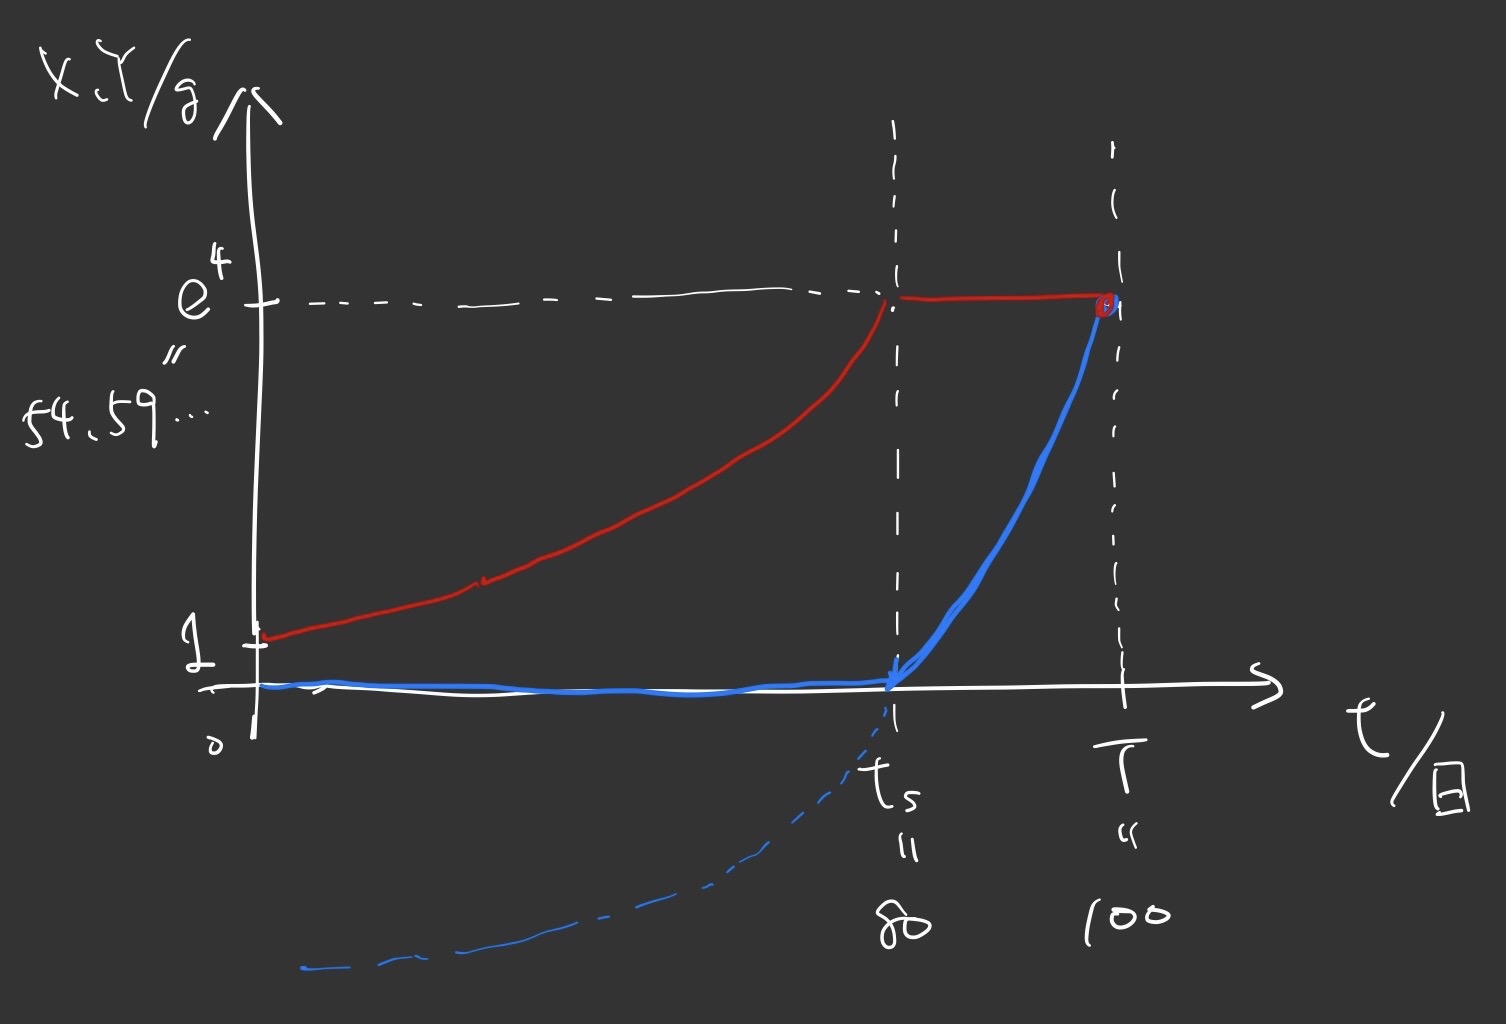
\includegraphics[width=17cm]{figure.JPG}
    \end{figure}
\end{center}

\subsection{小問3}

芋の方が,同じ個体を再生産できる上に,多くの栄養を貯蓄しているために環境条件が揃わないことによって種子が発芽できないなどのリスクが少ない.
一方で,無性生殖であるから,同一個体が長く生存するに従って有害な突然変異が蓄積する危険性がある.

このような場合に,種子であれば,有性生殖であるから遺伝子は刷新され,また突然の環境の変異などに対応できるような遺伝子の多様性を生み出すことができる.

\begin{thebibliography}{99}
        \bibitem{坂和愛幸}
        『最適制御理論におけるポントリャーギンの最大原理』坂和愛幸.計測と制御,1962.
        \bibitem{Optimal growth schedule of deciduoustree seedlings}
        "Optimal growth schedule of deciduoustree seedlings" M.TATENO and N. VVATANABE. Functional Ecology, 1988,2,89-96.
        \bibitem{Shoot/root balance of plants: Optimal growth of a system with many vegetative organs}
        "Shoot/root balance of plants: Optimal growth of a system with many vegetative organs" Yoh Iwasa, and Jonathan Roughgarden. 
        Theoretical Population Biology. Volume 25, Issue 1, February 1984, Pages 78-105. 
\end{thebibliography}

\end{document}